\documentclass[a4paper]{article}
\usepackage[utf8x]{inputenc}
\usepackage[brazil]{babel}
\usepackage[T1]{fontenc}
\usepackage{graphicx}
\usepackage{indentfirst}

\begin{document}

\begin{titlepage}
 \vfill
  \begin{center}
   {\large \textbf{CENTRO UNIVERSITÁRIO SENAC}} \\
   {\large \textbf{BACHARELADO EM CIÊNCIA DA COMPUTAÇÃO}} \\[4cm]
   
   {\large \textbf{GABRIEL VIEIRA FIGUEIREDO TOMAZ}}\\
   {\large \textbf{TALES CARLOS DE PÁDUA}}\\
   {\large \textbf{VINICIUS DE CARVALHO}}\\[4cm]


   {\Large Mini Games com Visão Computacional}\\[4cm]

\vspace{2cm}
\large \textbf{SÃO PAULO}

\large \textbf{MAIO DE 2014}
\end{center}
\end{titlepage}

\break

\begin{titlepage}
 \vfill
  \begin{center}
   {\large \textbf{CENTRO UNIVERSITÁRIO SENAC}} \\
   {\large \textbf{BACHARELADO EM CIÊNCIA DA COMPUTAÇÃO}} \\[4cm]

   {\large \textbf{Gabriel Vieira Figueiredo Tomaz, Tales Carlos de Pádua, Vinicius de Carvalho.}}\\ [1cm]
  
   {\large \textbf{viera\_frifri@hotmail.com, talescpadua@gmail.com, carvalho.v@outlook.com.}}\\ [3cm]
   
 
   {\Large Mini Games com Visão Computacional}\\[2cm]

   \hspace{.45\textwidth} 
   \begin{minipage}{.5\textwidth}
   \large "Pequenos jogos eletrônicos utilizando conhecimentos de Visão Computacional apresentados para a conclusão da disciplina Projeto Interativo III, do bacharelado em Ciência da Computação, Centro Universitário Senac."\\[0.5cm]
      Sob orientação do Prof.º: Marcelo Hashimoto
  \end{minipage}
  \vfill

\vspace{1cm}
\large \textbf{SÃO PAULO}

\large \textbf{MAIO DE 2014}
\end{center}
\end{titlepage}




\section{Resumo}


Conforme proposto na disciplina de Projeto Interativo III, a partir do estudo de algoritmos relacionados à visão computacional foram desenvolvidos pequenos jogos eletrônicos (mini games) em linguagem C usando a interface gráfica provida pela biblioteca Allegro 5 e uma interface de acesso à câmeras de vídeo provida pela biblioteca OpenCV, de modo que a visão computacional oferecesse não apenas uma opção de controle para o jogador, mas sim um diferencial na experiência e imersão do usuário ao vivenciar os mini games.\\

Palavras-chave: jogos eletrônicos, visão computacional, Allegro 5.\\  



\section{Abstract}


As proposed by the Interactive Project III discipline, from the study of algorithms related to computer vision were originated little eletronic games (mini games) in C language utilizing a graphical interface provided by Allegro 5 library and a web cam access interface provided by OpenCV library, in order to make computer vision offer not only another controller option for the player, but a different experience and imersion for the user while playing the mini games.\\

Keywords: eletronic games, computer vision, Allegro 5.\\



\section {Introdução}


A visão computacional é uma ciência e tecnologia voltada a lidar com a forma como as máquinas enxergam o mundo ao seu redor. As informações captadas por meio de sensores (como scanners, câmeras de vídeo, etc.) podem ser modeladas de diversas formas a fim de suprir necessidades que permeiam desde ramos diretamente ligados à tecnologia de informação (como robótica e áreas de automação tecnológica) até os que se utilizam da tecnologia para dadas outras necessidades, como ciências ambientais, medicina e outros.\\

Com o objetivo de dar um passo inicial para dentro da visão computacional, este trabalho visa utilizar técnicas e algoritmos da mesma aliada à captação de imagens por câmera de vídeo para a produção de jogos simples, mas que mantenham a jogabilidade focada no poder da visão computacional, de modo que a experiência do jogador, ao invés de ser restringida pela interface proposta, se torne um diferencial por conta deste quesito.



\section{Desenvolvimento}



\subsubsection{Ponto de Partida}


Visto que este trabalho foi o primeiro contato formal com a visão computacional por parte do grupo, a estatégia adotada desenvolver os mini games foi uma via de mão-dupla passando por um \textit{brainstorm} de jogos existentes até quais algoritmos poderiam modelar uma interface de controle aceitável para os mesmos e fazendo o caminho de volta, onde eram estudados algoritmos existentes e se imaginava o que era possível, em termos de jogos, produzir a partir deles.

A partir desta metodologia aliada à orientação e pesquisa, surgiram as tecnicas e algoritmos a seguir e a consequente combinação dos mesmos para elaboração dos jogos. 

No início do trabalho foi introduzido uma biblioteca, baseada em OpenCV, que faz a interface de acesso à câmera de maneira bem restrita, possibilitando apenas que houvesse contato com os quadros capturados da câmera fornecidos por uma matriz tridimensional onde a primeira dimensão é a altura (em pixels) da imagem, a segunda representa a largura (também em pixels) e a terceira são os componentes vermelho (red), verde (green) e azul (blue), respectivamente, do espaço de cores RGB. Todos os valores da matriz representam um número entre 0 e 255 do padrão RGB.


\subsubsection{ Jogo Genius}


Esse jogo consiste em um remake do classico jogo genius com a jogabilidade alterada para ser possivel jogar com imagens coloridas capturadas pela web cam.

A principal ideia do jogo se baseou inicialmente no reconhecimento básico da cor vermelha, onde se era verificado se o componente R do pixel era maior que a soma dos outros dois G e B, conseguindo detectar com sucesso a cor desejada. Apesar de funcionar relativamente bem para detecção de vermelho, outras cores apresentavam uma resistência maior ao método devido a pequenas instabilidades e mudanças de luz. Sendo necessário buscar algum outro método que pudesse fornecer uma melhor precisão nesse reconhecimento. Dentre alguns pesquisados, a solução adotada foi a conversão do espaço de cor RGB para o HSV, pois ele permite definir um range e uma intensidade para a detecção de uma cor especifica, ficando assim muito mais preciso devido suas caracteristicas únicas.


\vspace{5.00mm}

\begin{center}
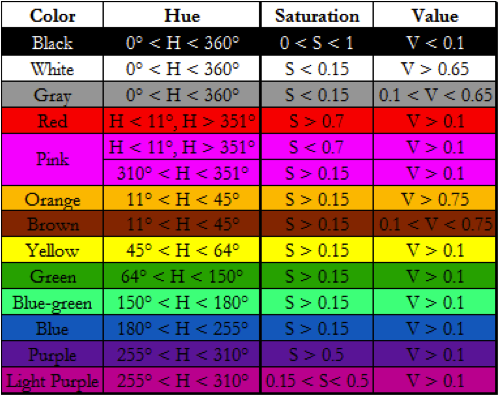
\includegraphics[scale=0.8]{scale.png} \\
\textbf{\normalsize Range das cores em HSV}
\end{center}


\begin{flushleft}
\textbf{\large Espaço de cor HSV}
\end{flushleft}
%%\raggedright


O sistema de cores HSV formadas pelas componentes Hue (tonalidade), Saturation (Saturação) e Value (Valor). Esse sistema também é conhecido como HSB (Hue, Saturation e Brightness - Tonalidade, Saturação e Brilho, respectivamente). A primeira componente H define a cor propriamente dita, podendo variar de 0 a 360 graus, a segunda componente S define a pureza ou intesidade da cor contida na componente H e por último a componente V defini o brilho da componente H.

\vspace{5.00mm}

\begin{center}
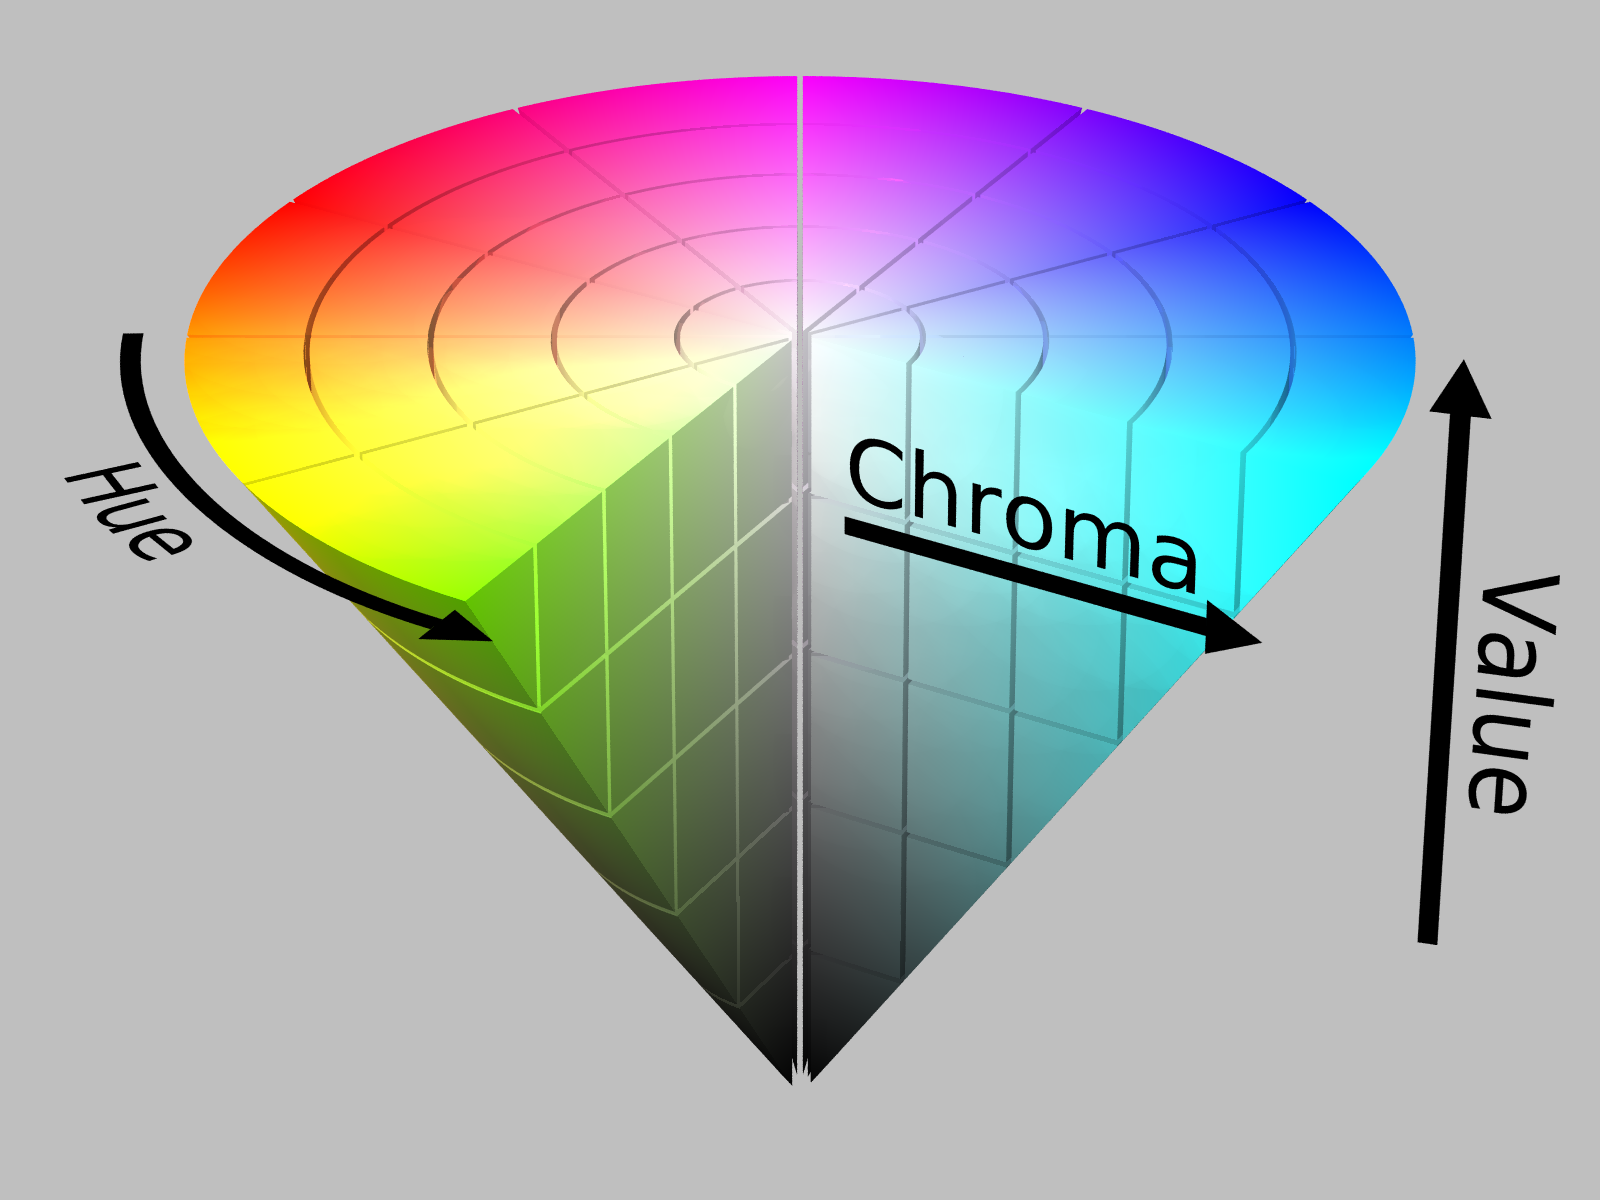
\includegraphics[scale=0.08]{hsv.png} \\
\textbf{\normalsize Espaço de cor HSV}
\end{center}
\vspace{5.00mm}


\begin{flushleft}
\subsubsection{Jogo: Sorvete Hoje?}
\end{flushleft}

%%\raggedright

A ideia deste jogo surgiu a partir do estudo de certos algoritmos que aliados permitem uma detecção de borda, que foi a base para a detecção de face. A detecção desta borda é feita por meio de um Filtro de Sobel, que será explicado mais adiante. Aliado ao filtro, para que houvessem bordas mais consistentes, foi utilizado um algoritmo de binarização de imagem. A técnica utilizada é conhecida como algoritmo de Otsu.

Apenas o filtro, porém, não era suficiente para atingir os objetivos, visto que a manipulação de quadros da câmera pode ser um processo bastante custoso, o que gera uma experiência ruim para o usuário. Visando um modo de se otimizar este processo, antes de se aplicar o algoritmo do filtro foi utilizada uma conversão da imagem para escala de cinza.

Por fim, para evitar impecilhos com a imagem de fundo da câmera, também foi agregado um algoritmo de remoção de fundo simples utilizando a fórmula matemática da Distância Euclidiana nos pixels dos quadros. \\

\subsubsection{Escala de Cinza}

O algoritmo de escala de cinza utilizado é bastante simples de ser aplicado no espaço de cor RGB, pois todos as cores obtidas ao se igualar as componentes R, G e B são tons de cinza. A fim de simplificar a quantidade de pixels que seriam processados, basta passar um algoritmo que soma as três componentes RGB de cada pixel, divide o valor por três e aplica o mesmo para as três componentes. Isto faz com que a imagem se torne descolorida com tons de cinza que são aproximações das cores da imagem original. Como as três componentes da terceira dimensão da matriz serão iguais, basta aplicar os algoritmos seguintes para apenas uma delas e replicar os resultados às demais, diminuindo assim a quantidade de processamento. \\

Fórmula para obter a escala de cinza:
$greyscale = \frac{R + G + B}{3}$ \\

Com cada componente R, G e B recebendo o valor de \textit{greyscale}.

\subsubsection{Filtro de Sobel}

O Filtro de Sobel calcula o gradiente da intensidade da imagem em cada ponto, dando a direção da maior variação de claro para escuro e a quantidade de variação nessa direção por meio de duas matrizes quadradas de ordem 3, que são convoluídas com a imagem original para calcular aproximações das derivadas. Uma das matrizes representa a variação horizontal $Gx$ e a outra é a vertical $Gy$. \\

\begin{center}{Máscara de Sobel 3x3}
$$
Gx=\left[\begin{array}{rrr}
-1&0&+1\\
-2&0&+2 \\
-1&0&+1
\end{array}\right]\quad
Gy=\left[\begin{array}{ccc}
-1&-2&-1\\
0& 0& 0 \\
+1&+2&+1
\end{array}\right]
$$
\end{center}

E a partir disto, calcula-se a magnitude do gradiente:

$$
|G|=\sqrt{Gx^2 + Gy^2}
$$  

A variação de claro para escuro indica a presença de uma borda e com este gradiente aplicado nos canais RGB tem-se uma imagem composta apenas pelas bordas dos objetos que a compõem. Como a imagem utilizada está em escala de cinza, o resultado é uma imagem composta de bordas claras (próximas ao branco) com massas escuras (que tendem ao preto).

\subsubsection{Binarização da imagem}

Apesar dos diversos algoritmos para binarização de imagem, como os quadros que estão sendo trabalhados já estão bastante simplificados neste ponto, uma implementação baseada no algoritmo de Otsu é suficiente para atingir o objetivo de itensificar as bordas obtidas no Filtro de Sobel.

A ideia geral do método de Otsu é ter um valor limite onde se atribui a cor branca para os pixels que possuírem o canal RGB acima deste limite e preto para os que estiverem abaixo do mesmo. Essa limítrofe em geral é calculada a partir de fórmulas que utilizam a imagem para definir qual seria o valor mais adequado, entretanto, para a imagem com bordas, pode-se definir um valor constante e simplificar todo o processo.

\subsubsection{Remoção de fundo com Distância Euclidiana}

Quando se quer ignorar o fundo de um determinado cenário, pode-se aplicar a distância entre dois pontos definida por Euclides como $dist(p, q) = \sqrt{p^2 - q^2}$ onde p e q são pontos com cordenadas $p_{1}, p_{2}, ... p_{n}$ e $q_{1}, q_{2}, ... q_{n}$. Capturando um quadro da câmera onde não há nada além do fundo do cenário, basta iterar entre todos os pontos (pixels) p deste quadro e os pontos q do quadro que se deseja remover o fundo. O resultado é uma imagem que exclui, de maneira simples, os elementos do cenário.

\subsubsection{Detecção de rosto}

O resultado de todos estes algoritmos alinhados é uma imagem de bordas bem definidas composta apenas pelo que não faz parte do cenário capturado pela câmera, ou seja, na grande parte dos casos haverá apenas a borda detalhada do jogador. O usuário é então instruído a posicionar seu rosto em um local específico onde é feito o reconhecimento facial, baseando-se no fato de que são esperados muitos pixels brancos para os olhos e a boca, mas poucos para a face visto que não há muitas bordas na mesma.

%\begin{figure}[!htb]
%\centering
%\includegraphics{tela_do_jogo.png}
%\caption{Figura 1 ? Tela do jogo com as cartas para a implementação dos algoritmos (Fonte: Jogo, Código de Honra criado pelo grupo ? Retirada 18/11/2013)}
%\label{Rotulo}
%\end{figure}

%\begin{figure}[!htb]
%\centering
%\includegraphics{git.png}
%\caption{Figura 2 ? Repositório do jogo criado para auxiliar o compartilhamento de dados via Web (Fonte: Github - https://github.com/tgl-dogg/BCC_PI2_CDH ? Retirada 20/11/2013)}
%\label{Rotulo}
%\end{figure}

\section{Resultados}

Os resultados obtidos com o desenvolvimente desse trabalho proporcionaram um algoritmo rústico de detecção de padroes da face e outro efeciente na detecção de cores, mostrando que com a combinação de alguns algoritmos simples de uma maneira inteligente é possivel chegar em grandes resultados. Resultados esses que podemos ver nos jogos criados que conseguem exercer seus objetivos com eficiencia e precisão.

Como resultado da convesão de espaço de cor pode-se ver um exemplo da detecção de azul:

\vspace{5.00mm}
\begin{center}
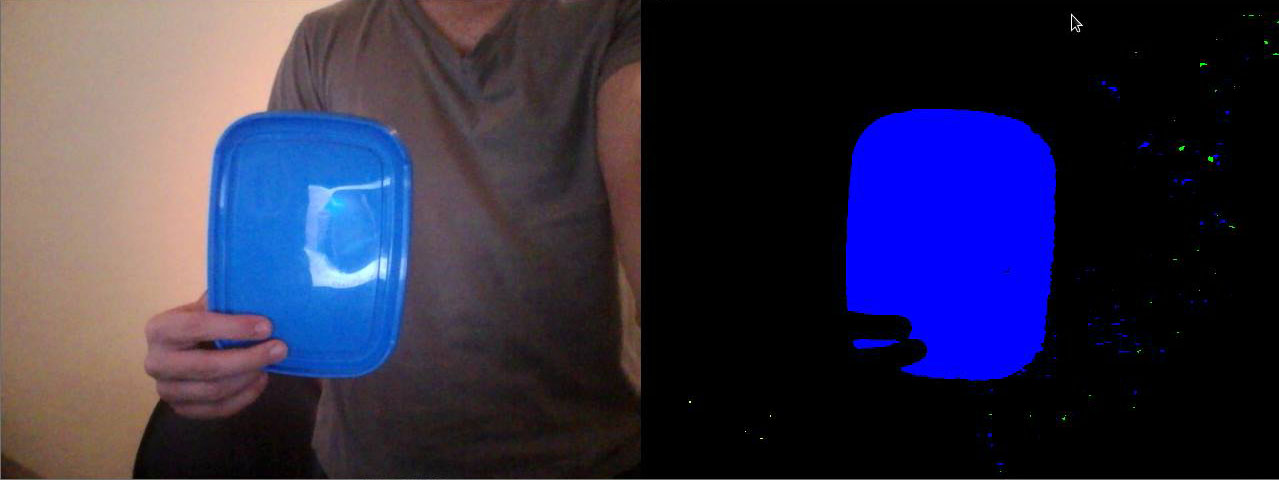
\includegraphics[scale=0.3]{img2.jpg}
\end{center}
\vspace{5.00mm}

E para a detecção de rosto, pode-se observar os resultados a seguir:

\vspace{5.00mm}
\begin{center}
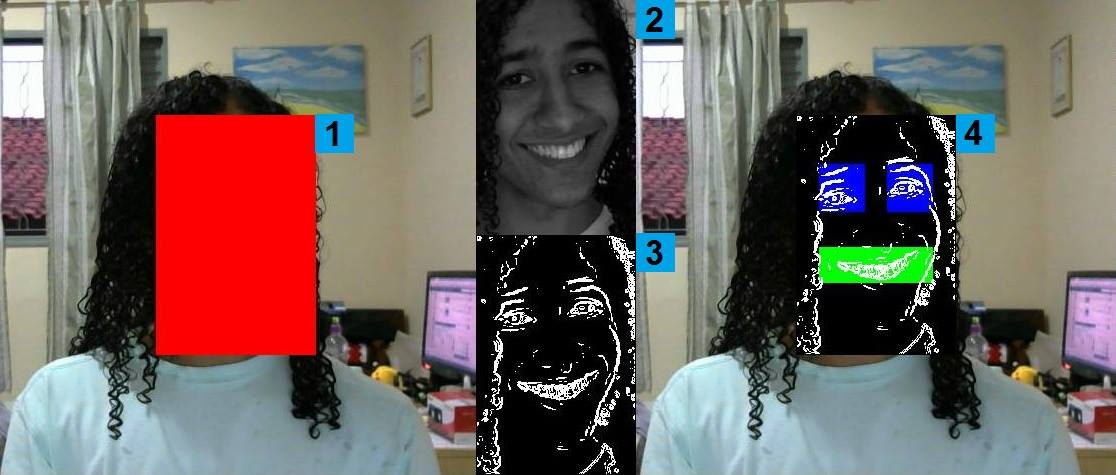
\includegraphics[scale=0.3]{img5.jpg}
\end{center}
\vspace{5.00mm}

À esquerda está a imagem original da câmera com um retângulo vermelho no item 1 indicando onde está a face do jogador.
O item 2 representa a face do jogador em escala de cinza antes de ser aplicado o Filtro de Sobel, e o item 3 representa o mesmo após a aplicação do filtro e da binarização.
O item 4 representa uma máscara que indica o local onde espera-se que o usuário posicione o rosto para que seja feito o reconhecimento do mesmo.

\section{Conclusão}


Existem diversas formas de se trabalhar com visão computacional e mesmo limitando o escopo de trabalho para produzir apenas jogos, foi possível estudar e aplicar conceitos bastante diferentes entre si, como mudanças de espaço de cor e métodos de tratamento de imagem para reconhecimento de padrões. Apesar de não serem as técnicas mais sofisticadas, todos os algoritmos descritos atenderam as necessidades de cada jogo e assim foi possível criar uma experiência de usuário realmente inovadora tanto para um jogo clássico, como o \textit{Genius}, quanto para um jogo independente, como o caso do \textit{Sorvete Hoje?}. 


\section{ Referências Bibliográficas}



\bibliographystyle{plain}
\begin{thebibliography}{2}

%link da biblioteca para aquisicao da camera
\bibitem{hashimoto}HASHIMOTO, Marcelo - Biblioteca fornecida para este projeto.
disponível em \url{https://github.com/senacbcc/Hashimoto-Camera-lib}.

%referencia do metodo de otsu    
\bibitem{Limiar}MATTEUCCI, Matteo. 
\newblock{Lecture 4 (2000), disponivel em}: 
\url{http://homepages.inf.ed.ac.uk/rbf/CVonline/LOCAL_COPIES/MORSE/threshold.pdf}. 

%minha principal referencia em processamento de imagem
\bibitem{procecimagens}
{MARQUES FILHO, Ogê; VIEIRA NETO, Hugo.}
\newblock {Processamento Digital de Imagens, Rio de Janeiro, Brasport, 1999.}

%referencia do sobel
\bibitem{Sobel1968}
{SOBEL, Irvin}
\newblock A 3x3 isotropic gradient operator for image processing.
\newblock Never published but presented at a talk at the Stanford Artificial
  Project, 1968.

\end{thebibliography}

\break

\end{document}